\documentclass{article}

% Environment setup

\usepackage[
    margin=.75in
]{geometry} %geometry (sets margin) and other useful packages 

\setlength{\parindent}{0em}
\setlength{\parskip}{.5em}

\usepackage{graphicx}
\usepackage{grffile}  % support extra dots in filenames
\usepackage{fancyref}
\usepackage[labelfont=bf]{caption}
\usepackage{subcaption}


\title{\textbf{CS 4641:} Unsupervised Learning and Dimensionality Reduction}
\author{Bradley Reardon}
\date{March 24, 2019}

\begin{document}
  \maketitle

  \section{Introduction}
    In this assignment, we are tasked with implementing two clustering algorithms and four dimensionality reduction algorithms, and seeing how they perform when applied both separately and together on two data sets. In addition, we'll take a focus on comparing these results to those of previous assignments when run on the same data sets. For comparison, all tests run for the purpose of this report will run each algorithm over 500 iterations, with a fixed seed to ensure reproducibility across tests.

    \subsubsection{Car data set}
      The Car Evaluation Database was created in June, 1997 by Marko Bohanec. It contains 1728 instances and 6 attributes. The purpose of this database is to attempt to classify a car as an unacceptable, acceptable, good, or very good choice based on factors including cost of ownership, comfort, and safety. Full details about the data set can be found at the source link below. Note that the instances of this data set completely cover the attribute space, making it an interesting problem for testing overfitting.

      \textbf{Source:} https://archive.ics.uci.edu/ml/datasets/car+evaluation

    \subsubsection{Breast Cancer Wisconsin data set}
      The Breast Cancer Wisconsin data set was donated to the UCI Machine Learning Repository in 1992, and contains data from one doctor's clinical cases, gathered from January 1989 to November 1991. In total, there are 699 instances signifying information about breast tumors such as clump thickness, uniformity in shape and size, and other screening factors. Data points are identified by two classes -- benign or malignant. The features of the data points are encoded as 9 continuous attributes rating the screening factor from 1 to 10.

      \textbf{Source:} https://archive.ics.uci.edu/ml/datasets/Breast+Cancer+Wisconsin+\%28Original\%29

  \section{Clustering}
    Clustering algorithms are a method for unsupervised learning which attempt to place a number of instances into clusters based on the closest mean of input attributes to an existing prototype. Because clustering would occur in either 6 or 9 dimensions, the main focus of analysis will be scoring the algorithms for each data set, though visualizations of these clusters do still show interesting information.

    \subsection{$k$-means Clustering}
      \subsubsection{Parameter selection}
        The main parameter for the $k$-means clustering algorithm is a value $k$, being the number of clusters that the algorithm will divide the data into. For both data sets, $k$ values of $2, 3, 4, 5, 6$ were tested for best performance. Each run of the algorithm used 20 initializations to ensure that the best possible cluster labelling is chosen for each data set. Smart initialization of clusters using the ``k-means++'' method ensure initial prototypes outperform random chance.

        The car data set did not perform very well in any of the $k$-means tests, with a maximum silhouette score of 0.119 being reported at a value of $k=3$. However, the data was known to be separated into 4 output classes, and the completeness of the instances over the attribute space led me to believe that a subset of the data may perform better.

        Running the algorithm again with only 500 of the 1728 total instances resulted in better silhouette scores overall, with the best performance occurring at $k=4$. \Fref{fig:km-silhouette-car} shows the silhouette plot and cluster visualization for this run.

        \begin{figure}[htb]
        \centering
        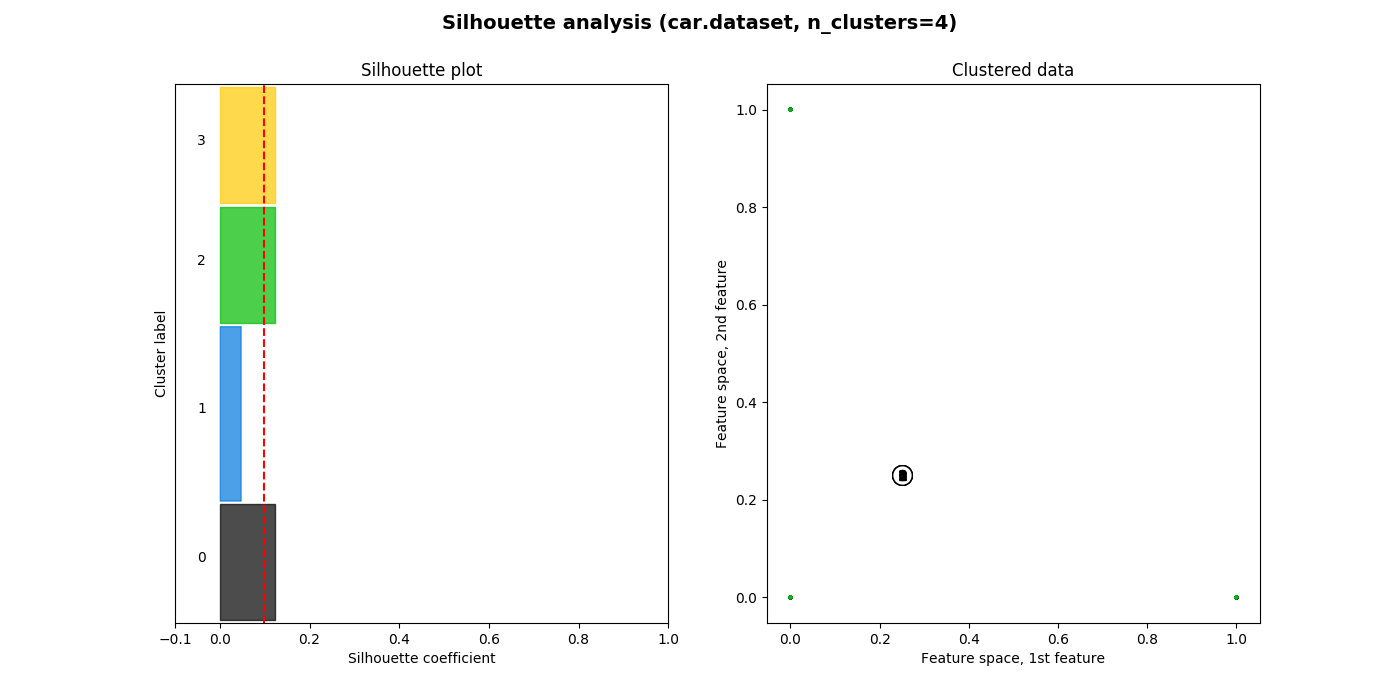
\includegraphics[width=\linewidth]{out/kmeans/car-4-clusters.png}
        \caption{Silhouette plot and clustered data visualization on two features for the car data set.}
        \label{fig:km-silhouette-car}
        \end{figure}

        The breast cancer data set was clustered better, with a best-performing $k=2$, matching the number of output classes. This resulted in a silhouette score of 0.577, which is much higher than that of the car data set. \Fref{fig:km-silhouette-cancer} shows the same visualizations for the cancer data set, which also reveals a very clear separation between the two clusters on the feature spaces for the first two features.

        \begin{figure}[htb]
        \centering
        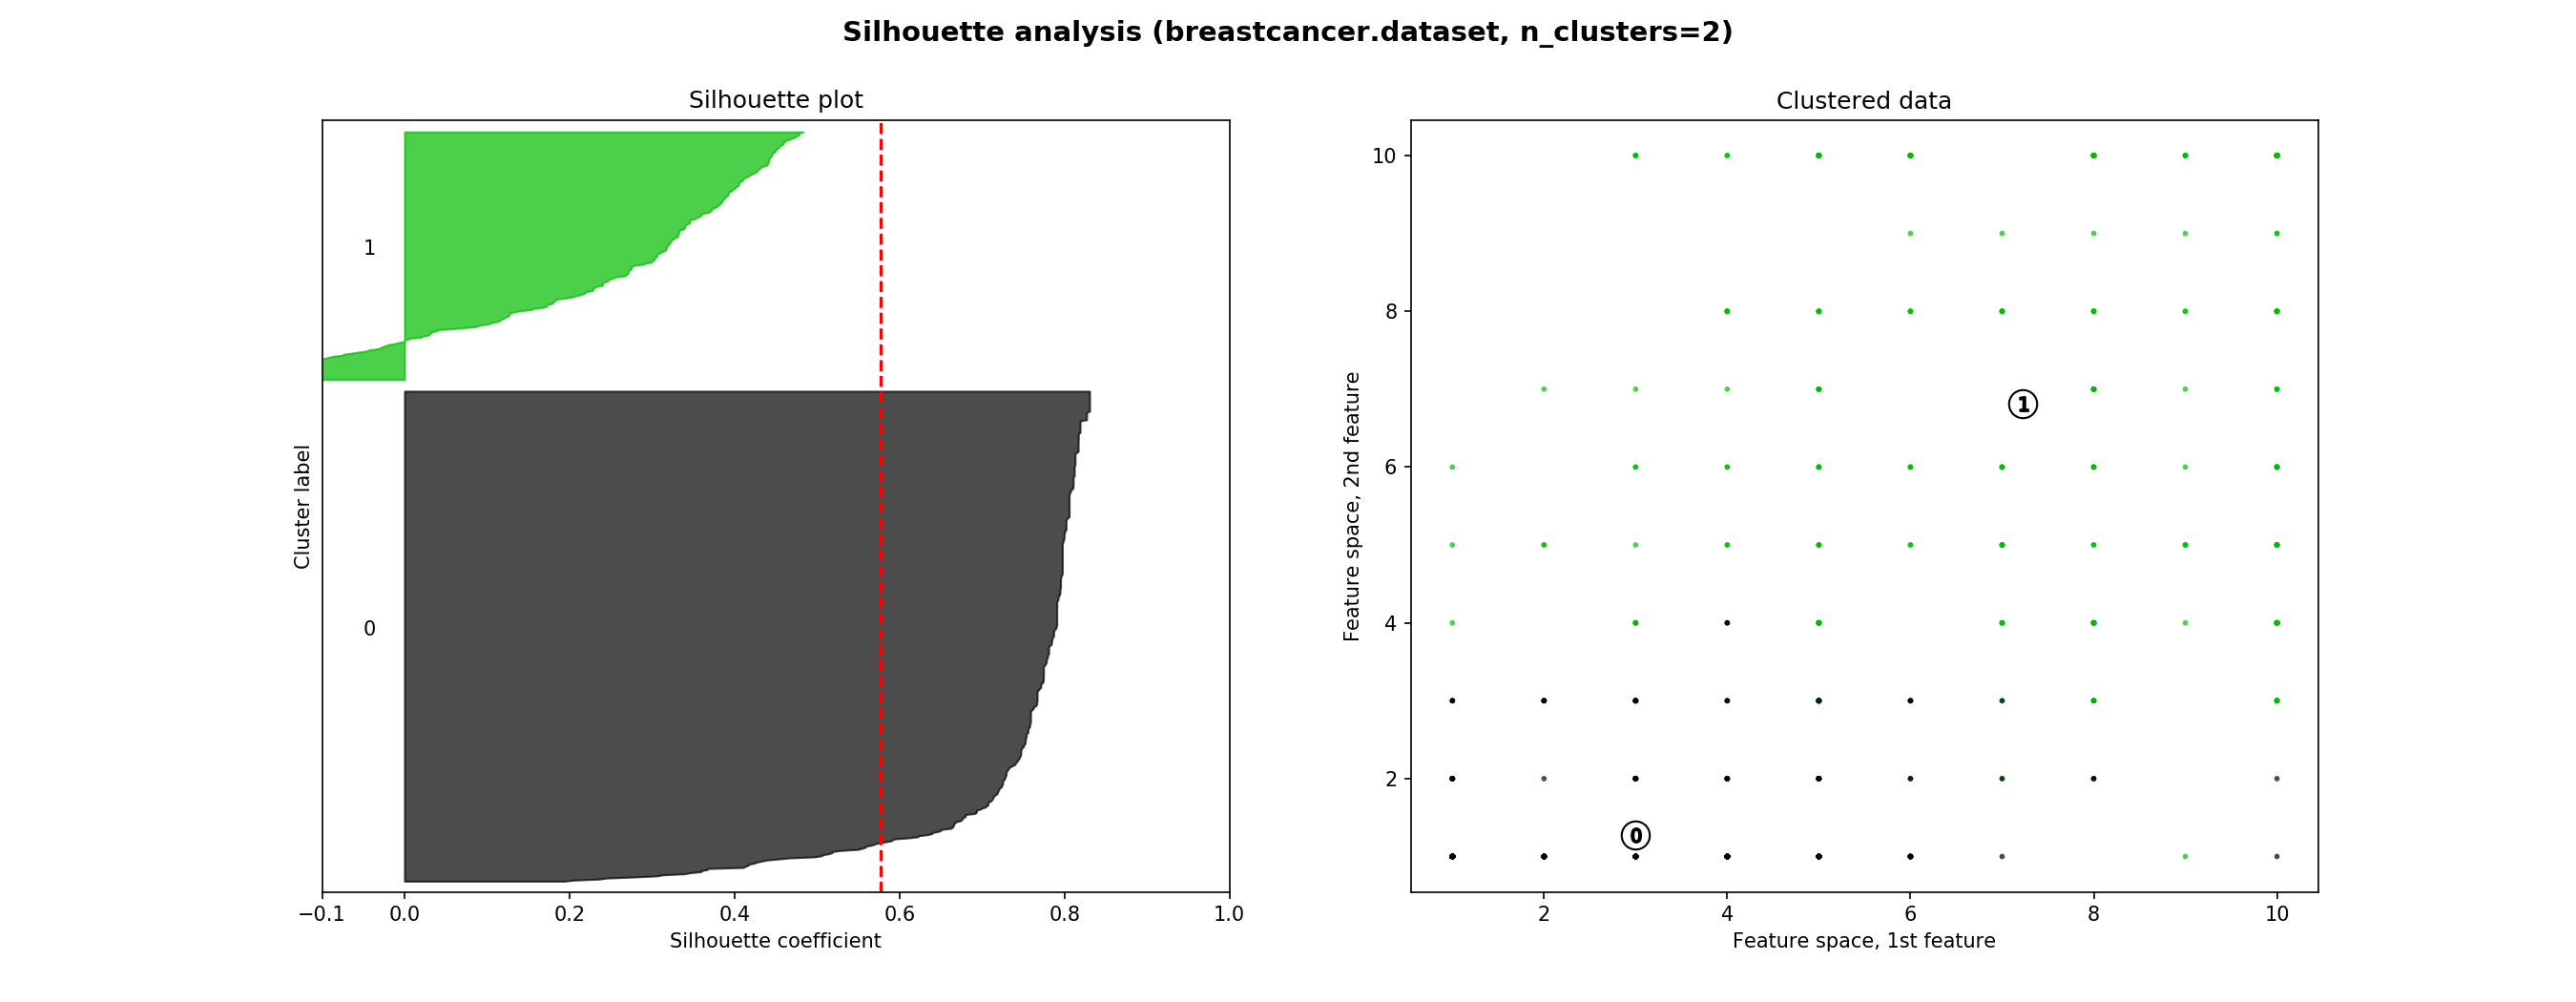
\includegraphics[width=\linewidth]{out/kmeans/cancer-2-clusters.png}
        \caption{Silhouette plot and clustered data visualization on two features for the cancer data set.}
        \label{fig:km-silhouette-cancer}
        \end{figure}

      \subsubsection{Performance}
        Using the ideal $k$ values of 4 and 2 for the cancer and car data sets respectively, learning curves were generated to evaluate the peformance over the two data sets. These curves can be found in \Fref{fig:kmeans-learning}.

        \begin{figure}[htb]
        \centering

          \begin{subfigure}{0.4\textwidth}
            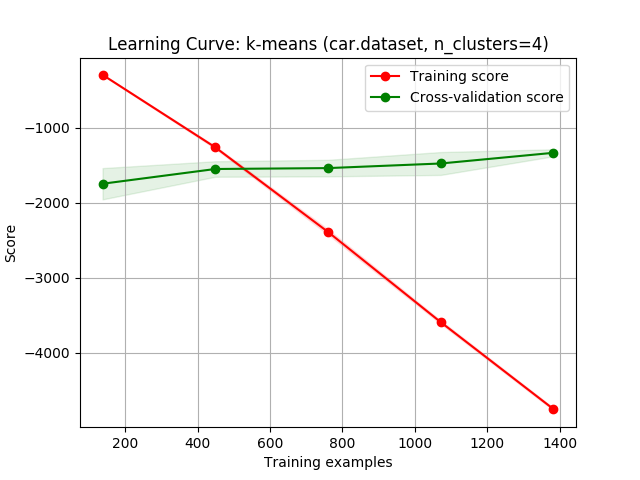
\includegraphics[width=\linewidth]{out/kmeans/car-learning.png}
            \caption{Learning curve, car.dataset}
            \label{fig:kmeans-learning-car}
          \end{subfigure}\hfil
          \begin{subfigure}{0.4\textwidth}
            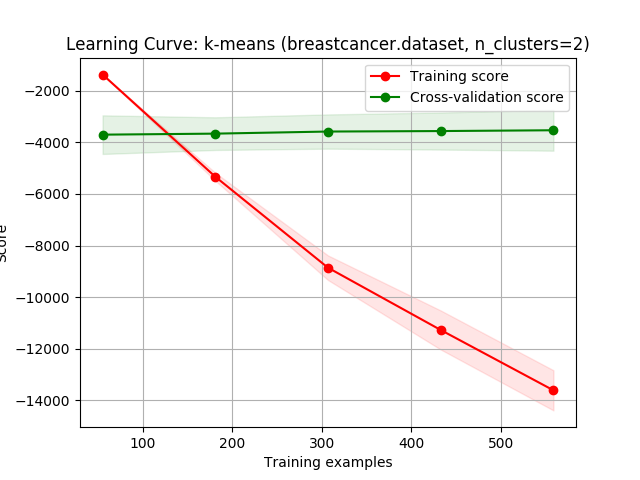
\includegraphics[width=\linewidth]{out/kmeans/cancer-learning.png}
            \caption{Learning curve, cancer.dataset}
            \label{fig:kmeans-learning-cancer}
          \end{subfigure}

        \caption{Learning curves for both data sets, using optimal parameters.}
        \label{fig:kmeans-learning}
        \end{figure}

        Both data sets seem to converge into clusters reasonably quickly, as shown by the low variance in the cross validation scores. Interestingly though, the variation in the car data set's cross validation score narrows as the proportion of training examples used approaches 100\%. The fit times of each test were recorded at 0.102s for the car data, and 0.044s for the cancer data. These running times will be compared to other algorithms and methods in a later section.

        Though the cancer data set is clustered better than the car data set by $k$-means, this same drop in variance is not observed. This suggests to me that the completeness of the instances in the car data had some effect on that outcome. However, this will be looked into further when dimensionality reduction algorithms are applied prior to clustering.

    \subsection{Expectation Maximization}
      The expectation maximization algorithm was tested using gaussian mixture models, with negative log-likelihood as the performance metric.

      \subsubsection{Parameter selection}
        Expectation maximization, in this implementation, takes one main parameter, which is the number of ``components''. Each algorithm was tested for best performance with between 1 and 15 components inclusive, as shown in \Fref{fig:em-comp}.

        \begin{figure}[htb]
        \centering

          \begin{subfigure}{0.4\textwidth}
            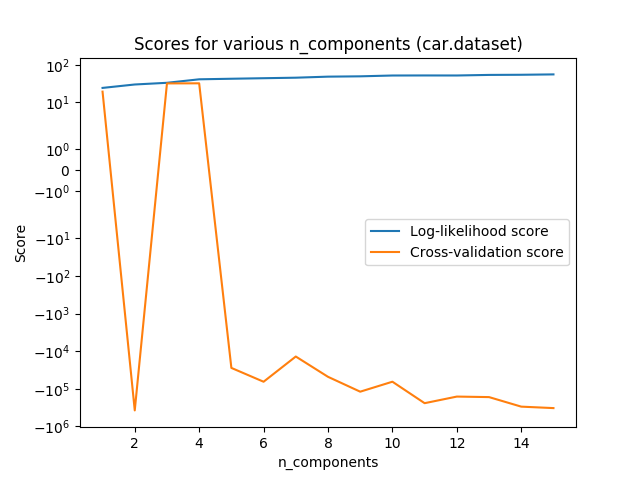
\includegraphics[width=\linewidth]{out/em/car-components-testing.png}
            \caption{Scores, car.dataset}
            \label{fig:em-comp-car}
          \end{subfigure}\hfil
          \begin{subfigure}{0.4\textwidth}
            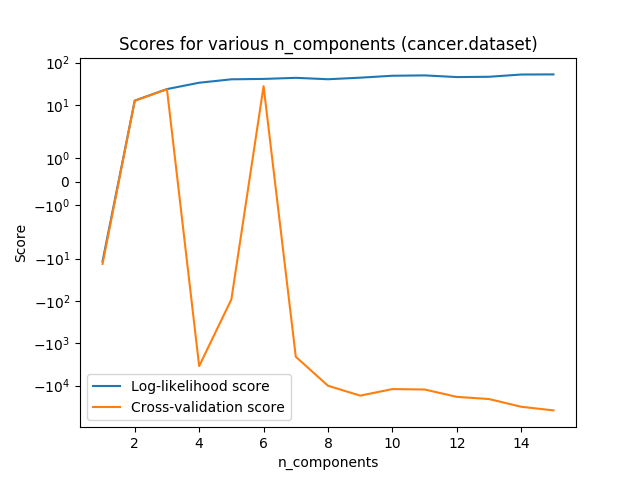
\includegraphics[width=\linewidth]{out/em/cancer-components-testing.png}
            \caption{Scores, cancer.dataset}
            \label{fig:em-comp-cancer}
          \end{subfigure}

        \caption{Log-likelihood of classifiers for both data sets with varying n\_components.}
        \label{fig:em-comp}
        \end{figure}

        In this case, the goal was to find the lowest number of components which resulted in the best scoring, as higher numbers of components increase running time. To satisfy this requirement, the car data set was chosen to have 4 components, while the cancer data set performed better with 3.

      \subsubsection{Performance}
        The learning curves for both data sets using expectation maximization are shown in \Fref{fig:em-learning}.

        \begin{figure}[htb]
        \centering

          \begin{subfigure}{0.4\textwidth}
            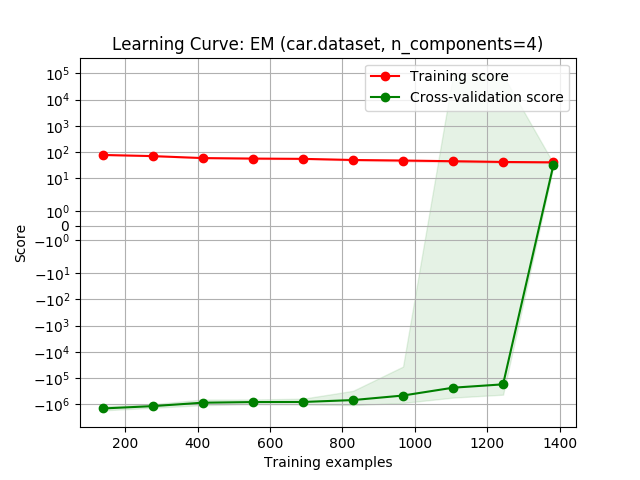
\includegraphics[width=\linewidth]{out/em/car-learning.png}
            \caption{Learning curve, car.dataset}
            \label{fig:em-learning-car}
          \end{subfigure}\hfil
          \begin{subfigure}{0.4\textwidth}
            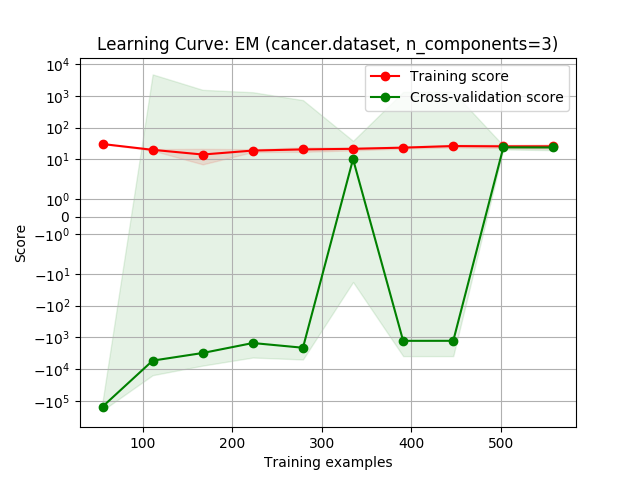
\includegraphics[width=\linewidth]{out/em/cancer-learning.png}
            \caption{Learning curve, cancer.dataset}
            \label{fig:em-learning-cancer}
          \end{subfigure}

        \caption{Learning curves for both data sets, using optimal parameters.}
        \label{fig:em-learning}
        \end{figure}

        The fit times for these classifiers were 0.025s for the car data, and 0.027s for the cancer data. Interestingly enough, both data sets have high variance in their cross validation scores at least at some point during training. In addition, the cancer data set seemes to have had its cross-validation score converge with the training scores at the end of training. This result will be discussed further after attempting dimensionality reduction.

  \section{Dimensionality Reduction}
    We will now evaluate dimensionality reduction algorithms, which are used for feature selection and to consolidate high-dimension datasets into data more easily digestible by machine learning algorithms. Note that with higher numbers of components, the dimensionality of the algorithm outputs is too high for 2D or 3D visualizations to be sufficient. As such, we will evaluate much of the performance of each algorithm on how it assists a clustering algorithm or a neural network in the next sections. This section will focus on identifying which dimensionality reduction algorithms are effective in clustering the data alone. 

    \subsection{PCA}
      \Fref{fig:pca-plot} shows the best-found configuration for PCA to maximize clustering apparent on the first two feature spaces. Interestingly, the cancer data set did not have any variation in PCA dimensionality reduction across the first two features of the data set. Due to the high-dimensionality of PCA with larger numbers of components, it is difficult to show the effectiveness of the PCA algorithm at higher numbers of components.

      As such, the car data set showed the most apparently clustering on two features with 4 components, whereas the cancer data set did not show any change in clustering on the first two features after adding more components.

      \begin{figure}[htb]
      \centering

        \begin{subfigure}{0.4\textwidth}
          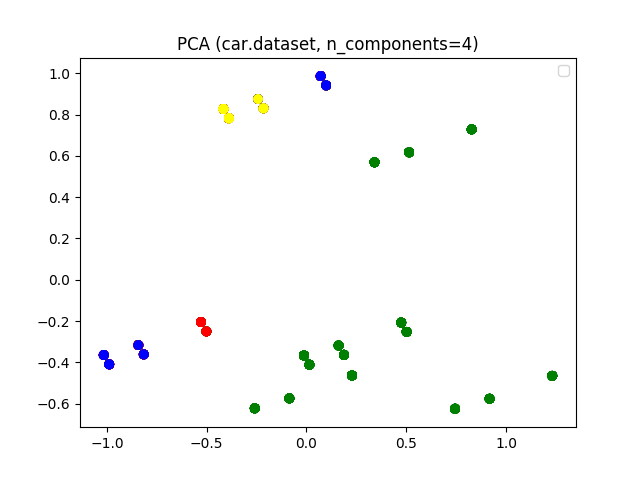
\includegraphics[width=\linewidth]{out/pca/car-pca-comp-4.png}
          \caption{PCA, car.dataset}
          \label{fig:pca-plot-car}
        \end{subfigure}\hfil
        \begin{subfigure}{0.4\textwidth}
          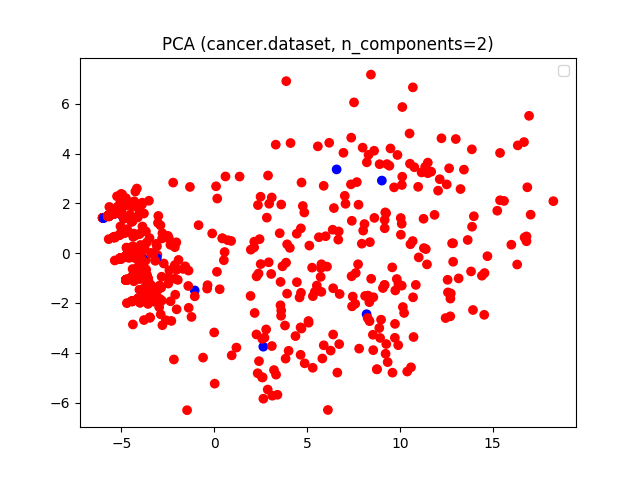
\includegraphics[width=\linewidth]{out/pca/cancer-pca-comp-2.png}
          \caption{PCA, cancer.dataset}
          \label{fig:pca-plot-cancer}
        \end{subfigure}

      \caption{PCA plots for both data sets.}
      \label{fig:pca-plot}
      \end{figure}

      TODO something more about variance/statistics from PCA

    \subsection{ICA}
      The ICA algorithm resulted in similar clustering to that of the PCA algorithm for the car data set, while clustering the cancer data into narrower bands that more effectively produced a cluster of blue points signifying the malignant tumor class. In this case, the number of components specified had a large effect on the plots of both data sets. The plots for the ICA algorithm can be seen in \Fref{fig:ica-plot}.

      \begin{figure}[htb]
      \centering

        \begin{subfigure}{0.4\textwidth}
          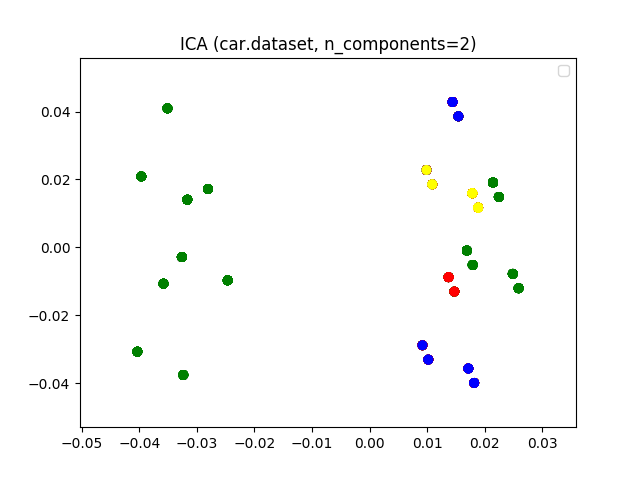
\includegraphics[width=\linewidth]{out/ica/car-ica-comp-2.png}
          \caption{ICA, car.dataset}
          \label{fig:ica-plot-car}
        \end{subfigure}\hfil
        \begin{subfigure}{0.4\textwidth}
          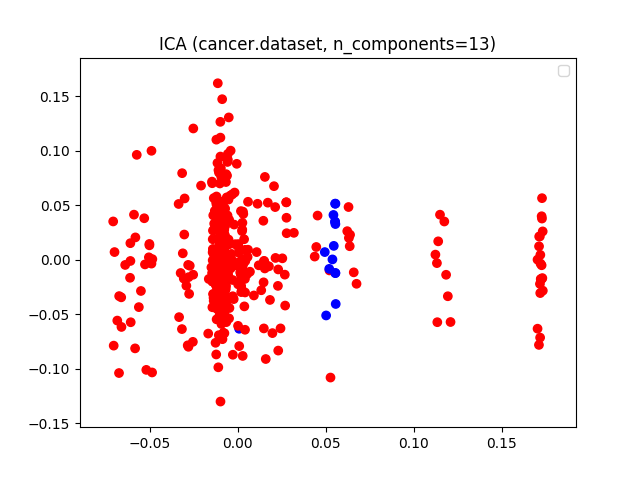
\includegraphics[width=\linewidth]{out/ica/cancer-ica-comp-13.png}
          \caption{ICA, cancer.dataset}
          \label{fig:ica-plot-cancer}
        \end{subfigure}

      \caption{ICA plots for both data sets.}
      \label{fig:ica-plot}
      \end{figure}

    \subsection{Randomized Projections}
      Unlike PCA and ICA, a run of randomized projections using the gaussian random projection algorithm from scikit-learn did not result in any meaningful clustering of either data set when plotted on two features, as shown in \Fref{fig:rp-plot}. The effectiveness of this algorithm on the data will be further evaluated when combined with another learner, such as a clustering algorithm or neural net.

      \begin{figure}[htb]
      \centering

        \begin{subfigure}{0.4\textwidth}
          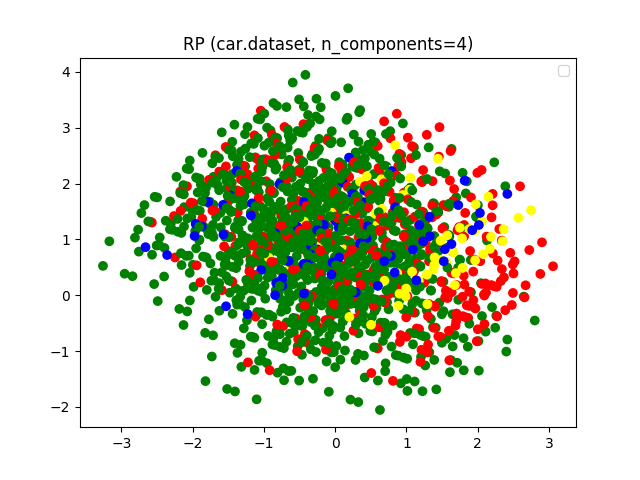
\includegraphics[width=\linewidth]{out/rp/car-rp-comp-4.png}
          \caption{RP, car.dataset}
          \label{fig:rp-plot-car}
        \end{subfigure}\hfil
        \begin{subfigure}{0.4\textwidth}
          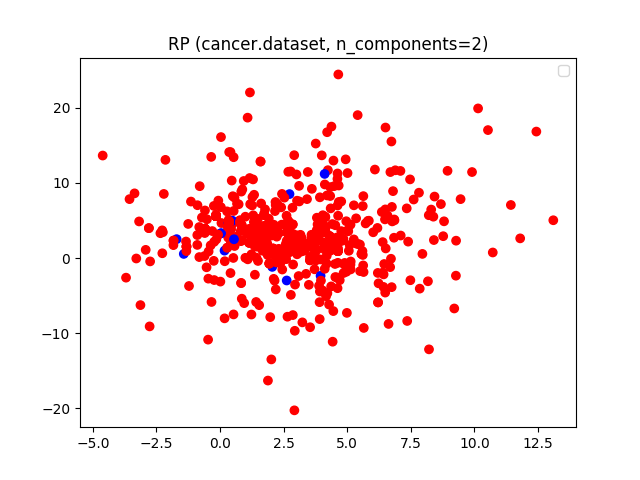
\includegraphics[width=\linewidth]{out/rp/cancer-rp-comp-2.png}
          \caption{RP, cancer.dataset}
          \label{fig:rp-plot-cancer}
        \end{subfigure}

      \caption{RP plots for both data sets.}
      \label{fig:rp-plot}
      \end{figure}

    \subsection{TODO pick feature selection algo??}
      TODO

  \section{Clustering with Dimensionality Reduction}
    Both the $k$-means clustering algorithm and expectation maximization algorithms were run with ICA and PCA for dimensionality reduction and compared to the standard clustering runs without dimensionality reduction.

    \Fref{fig:cdr-plot-km-car} and \Fref{fig:cdr-plot-em-car} show the differences (or rather lack thereof) in the learning curves between the various runs with no dimensionality reduction, and with ICA and PCA. For the car dataset, dimensionality reduction had no discernable effect on the learning curve, further confirming the earlier hypothesis that such a complete covering of the attribute space does not gain any extra performance or information from reducing the dimensionality of the data.

    In addition, both randomized projection and feature agglomeration were used for further attempts at dimensionality reduction, however again no discernable difference was found.

    \begin{figure}[htb]
    \centering

      \begin{subfigure}{0.33\textwidth}
        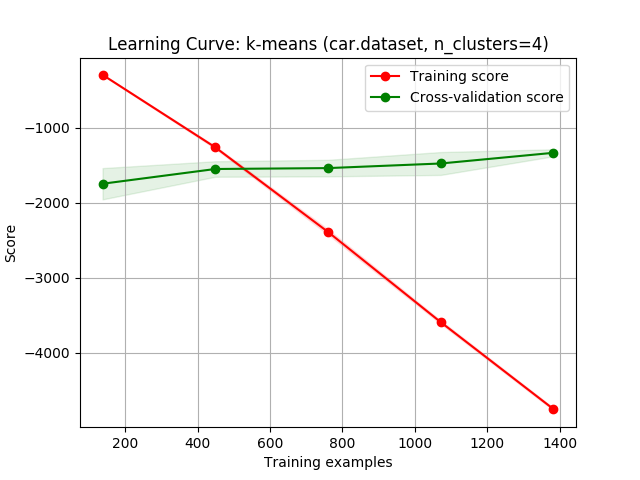
\includegraphics[width=\linewidth]{out/kmeans/car-learning.png}
        \caption{No DR, car.dataset}
      \end{subfigure}\hfil
      \begin{subfigure}{0.33\textwidth}
        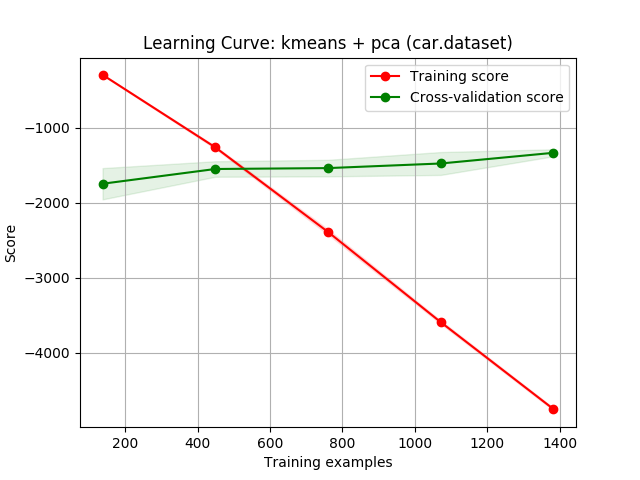
\includegraphics[width=\linewidth]{out/cluster_dr/car-kmeans-pca-learning.png}
        \caption{PCA, car.dataset}
      \end{subfigure}\hfil
      \begin{subfigure}{0.33\textwidth}
        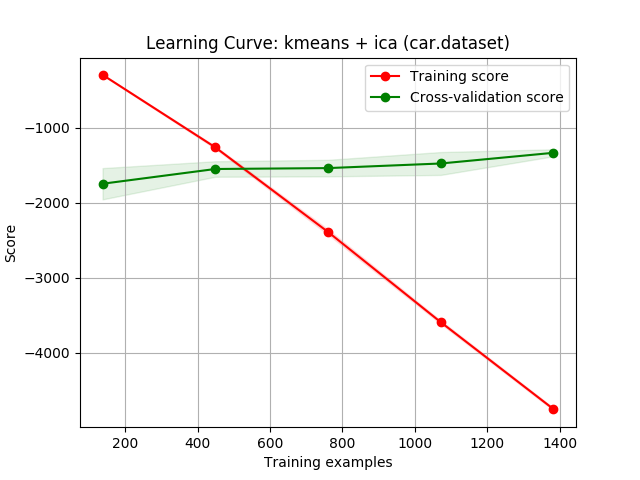
\includegraphics[width=\linewidth]{out/cluster_dr/car-kmeans-ica-learning.png}
        \caption{ICA, car.dataset}
      \end{subfigure}

    \caption{$k$-means clustering, car.dataset}
    \label{fig:cdr-plot-km-car}
    \end{figure}

    \begin{figure}[htb]
    \centering

      \begin{subfigure}{0.33\textwidth}
        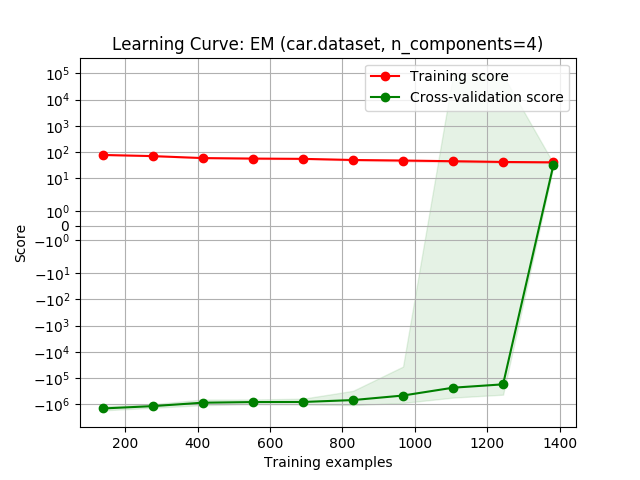
\includegraphics[width=\linewidth]{out/em/car-learning.png}
        \caption{No DR, car.dataset}
      \end{subfigure}\hfil
      \begin{subfigure}{0.33\textwidth}
        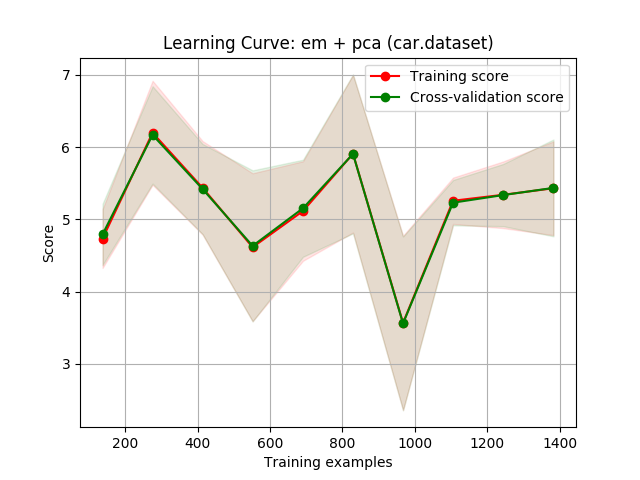
\includegraphics[width=\linewidth]{out/cluster_dr/car-em-pca-learning.png}
        \caption{PCA, car.dataset}
      \end{subfigure}\hfil
      \begin{subfigure}{0.33\textwidth}
        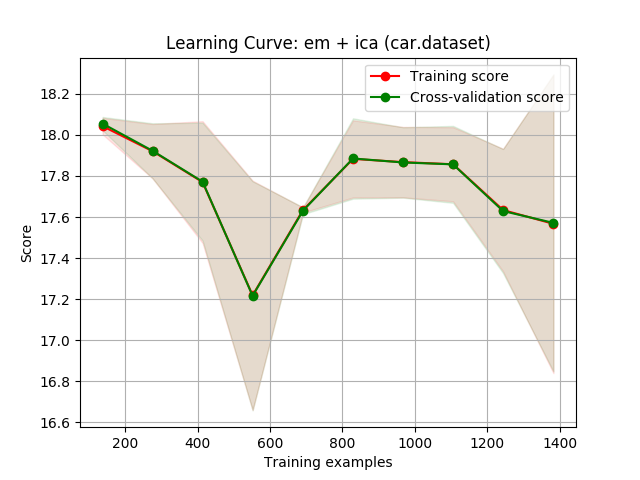
\includegraphics[width=\linewidth]{out/cluster_dr/car-em-ica-learning.png}
        \caption{ICA, car.dataset}
      \end{subfigure}

    \caption{Expectation maximization, car.dataset}
    \label{fig:cdr-plot-em-car}
    \end{figure}
    
    \Fref{fig:cdr-plot-km-cancer} and \Fref{fig:cdr-plot-em-cancer} show the same results for running clustering algorithms along with or without dimensionality reduction, however this time on the breast cancer data set. For the $k$-means clustering algorithm, the cross-validation score reported with dimensionality reduction was much lower than in the case of running clustering without DR. However, while running expectation maximization, the effects of using any form of dimensionality reduction are less pronounced.

    The resulting plot with $k$-means clustering and dimensionality reduction on the cancer data is indicative of DR having a positive effect on the clustering algorithm. Namely, it seems that using DR allowed the $k$-means clustering algorithm to filter out noise by grouping together attributes that have relationships.

    \begin{figure}[htb]
    \centering

      \begin{subfigure}{0.33\textwidth}
        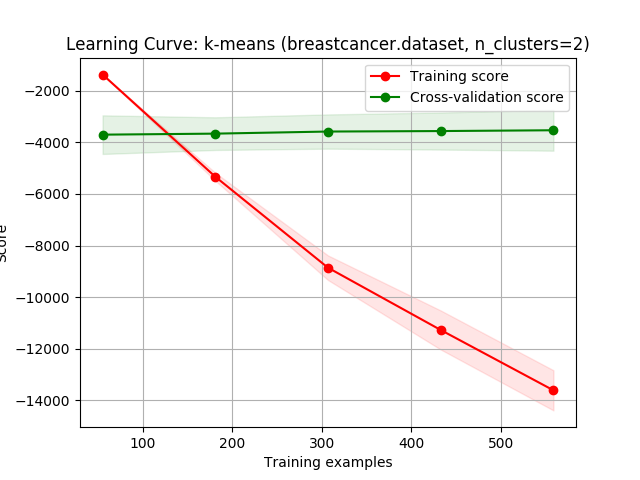
\includegraphics[width=\linewidth]{out/kmeans/cancer-learning.png}
        \caption{No DR, cancer.dataset}
      \end{subfigure}\hfil
      \begin{subfigure}{0.33\textwidth}
        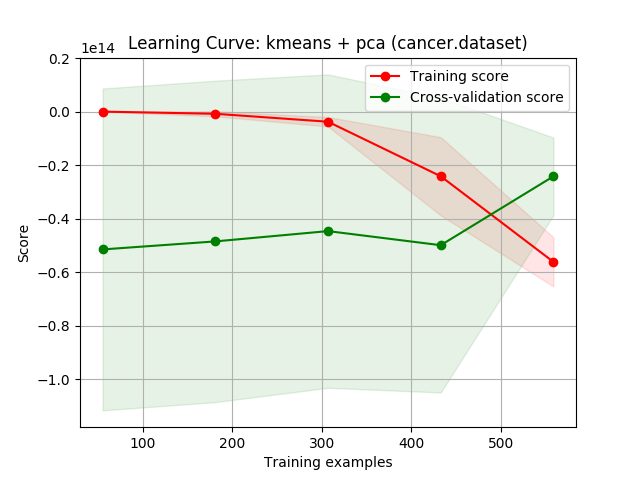
\includegraphics[width=\linewidth]{out/cluster_dr/cancer-kmeans-pca-learning.png}
        \caption{PCA, cancer.dataset}
      \end{subfigure}\hfil
      \begin{subfigure}{0.33\textwidth}
        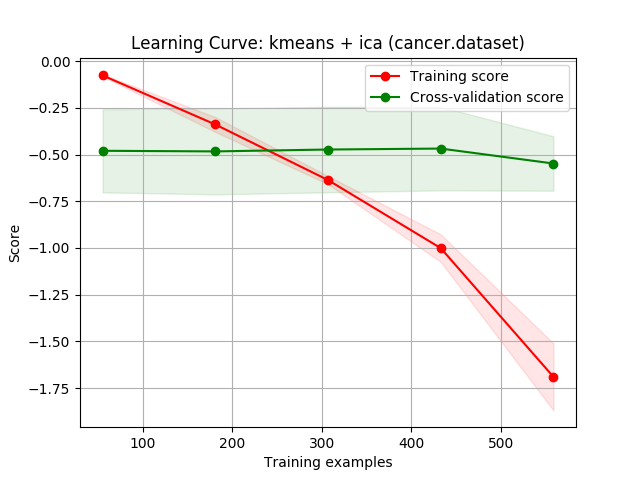
\includegraphics[width=\linewidth]{out/cluster_dr/cancer-kmeans-ica-learning.png}
        \caption{ICA, cancer.dataset}
      \end{subfigure}

    \caption{$k$-means clustering, cancer.dataset}
    \label{fig:cdr-plot-km-cancer}
    \end{figure}


    \begin{figure}[htb]
    \centering

      \begin{subfigure}{0.33\textwidth}
        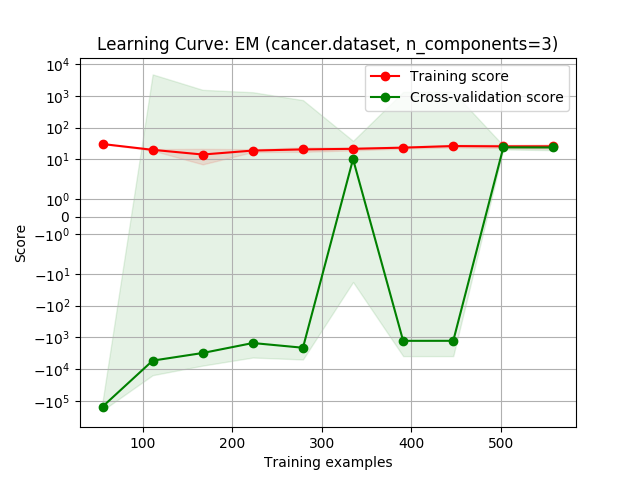
\includegraphics[width=\linewidth]{out/em/cancer-learning.png}
        \caption{No DR, cancer.dataset}
      \end{subfigure}\hfil
      \begin{subfigure}{0.33\textwidth}
        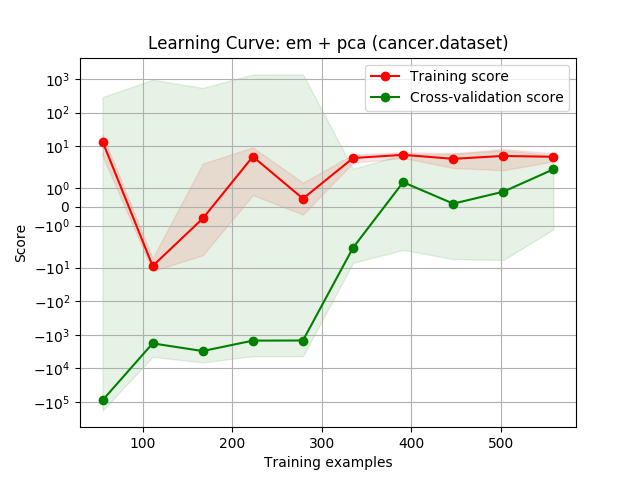
\includegraphics[width=\linewidth]{out/cluster_dr/cancer-em-pca-learning.png}
        \caption{PCA, cancer.dataset}
      \end{subfigure}\hfil
      \begin{subfigure}{0.33\textwidth}
        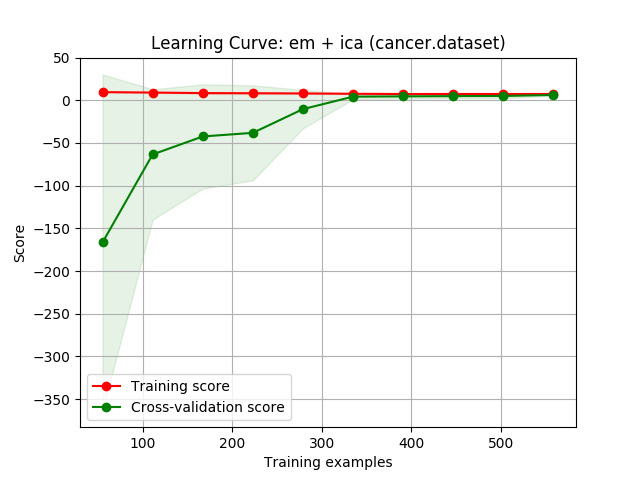
\includegraphics[width=\linewidth]{out/cluster_dr/cancer-em-ica-learning.png}
        \caption{ICA, cancer.dataset}
      \end{subfigure}

    \caption{Expectation maximization, cancer.dataset}
    \label{fig:cdr-plot-em-cancer}
    \end{figure}

  \section{Conclusion}
    TODO DR seems mostly ineffective on my data sets, perhaps improvements in some cases, but too few features to really make sense of if it's helping 

    Relate two assignments 1/2



\end{document}